\part{Introduction}

\chapter{Introduction}

What has been one of the main dangers humanity has faced throughout its history? The first answers that can be given are war or climate change, but there is another great threat that has severely affected the lives of almost all human populations over time: diseases and epidemics. There were no periods - not in the past, nor nowadays - when illnesses didn't influence human lives. 

Looking at the past, the consequences of epidemics on the population were worse than today, mostly because of the lack of knowledge about medical science and the poor hygienic conditions. During the bubonic plague of the 14th century, for example, 25 million deaths were reported in Europe out of a population of 100 million. The pandemic also triggered social unrest: Jews were considered responsible for the illness spread and they began to be persecuted: there were several attacks and massacres to the Jewish communities in different European cities, like Toulon, Barcelona, Erfurt, Basel, Frankfurt, Strasbourg. The persecution mainly was related to belief that Jews were less affected by the disease, and that were responsible of the poisoning of wells.
\begin{figure}[ht]
	\centering
	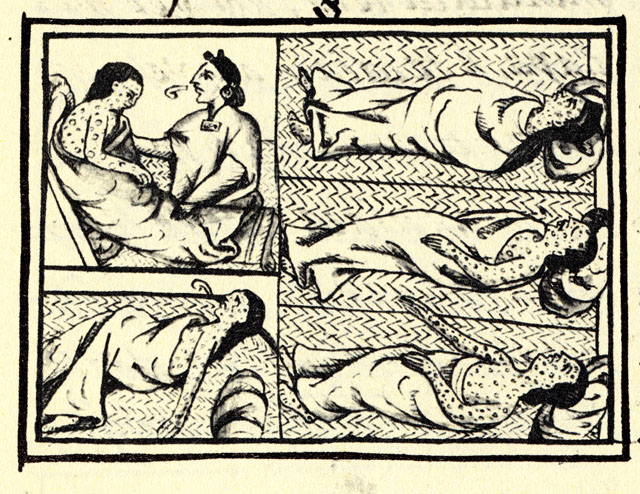
\includegraphics[width=0.43\linewidth]{0_introduction/images_introduction/FlorentineCodex_smallpox}
	\caption[Smallpox on native Americans]{Representation of smallpox disease on the Mexican population in the $XIV$ century. Figure from the Florentine Codex \cite{Sahagun1965}. }
	\label{fig:florentinecodexsmallpox}
\end{figure}
\\
\newpage
Another example is how during the course of the Americas' colonization, the diseases imported by the Europeans were one of the main causes of the genocide of the local population, largely contributing to their defeat against the Spanish conquistadors. In fact, diseases like smallpox and cholera were unknown in these countries and native Americans had no antibodies to contrast them. 
Other important epidemics, famous for their consequences, were the Spanish influenza, Smallpox, Typhus, HIV/AIDS, and the more recent COVID-19. 
It is straightforward to notice the effect that diseases have on our lives.

The development of modern medicine and hygiene contributed to enhancing the quality of life. An example of this is that only in the last three centuries and especially in the most economically developed countries, a significant increase in life expectancy has been observed \cite{Anderson_82}.
This increase is also happening in poorer regions, such as Sub-Saharan Africa. Although their current life expectancy is lower than that of wealthier countries, recent research \cite{Vollset_2024} predicts a significant rise over the next 30 years. This study also forecasts that this trend will lead to a global convergence in life expectancy between now and 2050.
The most plausible explanation for this future prediction is that improvements in healthcare levels lead to changes in the causes of mortality as nations' wealth increases. In poorer regions, the primary causes of death are communicable, maternal, neonatal, and nutritional diseases, whereas in more developed and wealthier countries, non-communicable diseases like cancer and cardiovascular conditions become the main causes of death \cite{eurostat}.

However, despite rising life expectancy, epidemics continue to be one of the most significant threats to populations. In fact, there was a notable increase in the frequency and magnitude of reported epidemics during the 19th and 20th centuries \cite{Anderson_82}. This makes it essential to develop effective policies to control and mitigate their impact, requiring coordinated implementation by countries within the same macro-region.
\begin{figure}[h]
	\centering
	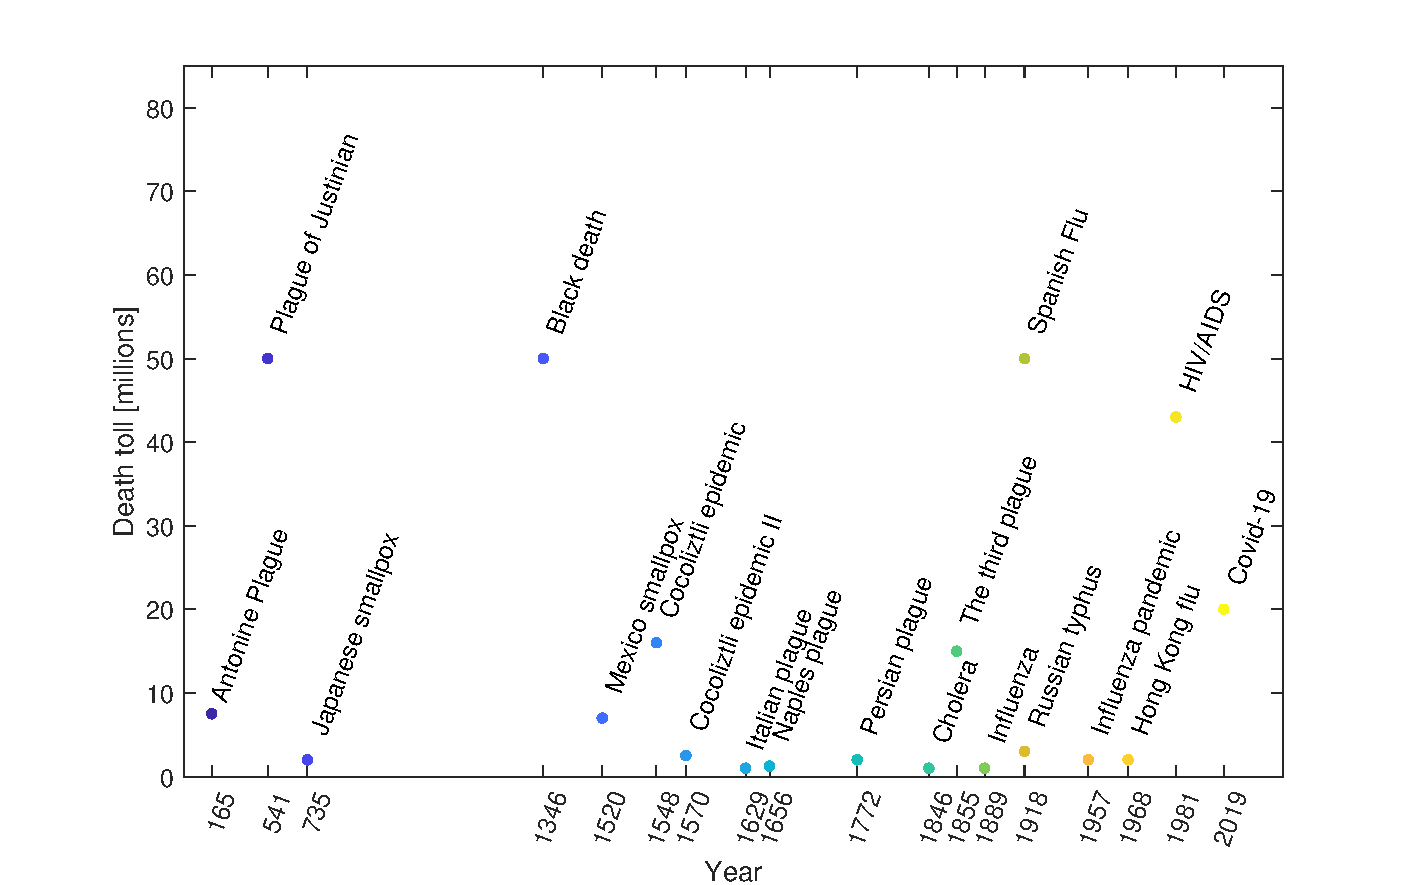
\includegraphics[width=0.95\linewidth]{0_introduction/images_introduction/worst_epidemic}
	\caption[Epidemic distribution in time]{A graphical representation of the distribution of known epidemics over the years and of their associated death toll. It is observable how there is an increment in the number of these event in the last three centuries. Data extracted from \cite{owid_historical_pandemics,wiki_pandemics}}
	\label{fig:worstepidemic}
\end{figure}

Figure \ref{fig:worstepidemic} highlights this trend. Although it becomes increasingly difficult to obtain reliable information about disease outbreaks the further back in time one goes, epidemics remain a tangible and present threat. This underscores the need for attention and action in shaping health policies that effectively address these dangers.
However, health status is not the only factor impacted by diseases. Illness can profoundly alter relationships, work, and social life, leading to a deterioration in overall social well-being as well \cite{Yang_2020}. 
There is also an economic cost associated with the cure. Only in a few nations worldwide, is treatment covered free of charge by the state. In the majority of countries, being ill can result in having to sustain high costs, causing people to go into debt or not take care \cite{esteban_2017, Barlow2021}. 
All these effects sum together and influence how populations behave when facing an epidemic. What are the consequences of adopting a certain behavior during a disease outbreak? It's a crucial question that can help to understand how to develop more efficient policies for contrasting epidemics. It is also the question that represents the first objective of study for the present work: How can a multidisciplinary model be developed that integrates elements from both social and epidemiological aspects to provide some insights into their mutual influence during the spread of a disease?
\\
\newline
Taking a step back, it's important to understand why epidemic models are crucial and what this field of research entails.
When a new disease emerges, the primary objective is to develop a defense against it. This begins with an epidemiological investigation to understand the disease's origin, the biological mechanisms behind its spread, and its resistance to existing drugs. The goal of this investigation is to gather all available information and understand the unfolding situation.
The next crucial step involves studying the dynamics of the disease and developing a predictive model for its evolution. This process requires understanding and estimating various parameters associated with the disease, including the transmission mechanisms within the population, the reproductive rate of the infectious agent, the acquisition and persistence of immunity, and the contagion mechanism.
Creating a reliable model is not only scientifically valuable but also serves as a powerful tool for stakeholders, helping to formulate effective policies during a pandemic emergency. Theoretical epidemiology aims to provide insights and policy recommendations in this context. Furthermore, data acquisition and analysis are essential for statistically modeling epidemic coefficients. 
Ultimately, a model that can address stakeholders' questions and make predictions—whether or not safety regulations are implemented—has significant implications for society. Beyond the economic costs associated with illnesses, there are also substantial social costs. Developing tools to understand better disease transmission can help mitigate its impact and alleviate the social burden, potentially saving numerous lives.
\\ \newline
A clear example of the potential benefits of having an epidemic model is the ability to generate synthetic insights that are easy to understand and can be expressed numerically. Such models can provide answers to critical questions like:
\begin{itemize}
	\item Is the disease so infective that can cause a pandemic?
	\item What are the threshold conditions that can cause an outbreak? 
	\item What is the expected number of infections over time?
\end{itemize}

At first glance, the problem may appear straightforward. However, the creation of a model capable of evaluating every disease remains an unsolved challenge.
Research in epidemic modeling requires striking a balance between simplification and maintaining accuracy. A good model effectively reproduces key phenomena with reasonable sophistication. While creating an overly complex model that attempts to incorporate every detail of a disease might be tempting, it often requires significant effort and data. In many cases, such models don't outperform simpler ones that focus on capturing the most important dynamics of disease spread. By prioritizing essential characteristics, simpler models can provide more practical insights while remaining computationally efficient.

Over the past century, various aspects of epidemics have been extensively studied. Notable achievements by scientists include:
\begin{itemize}
	\item Development of epidemiological models using different mathematical tools, such as differential equations, networks or agent-based models \cite{Hernandez_Vargas_2022, Keeling_2005}.
	\item Predictions about the progression of epidemics or reconstructions of the events' dynamics \cite{diekmann2000mathematical, brauer2012mathematical, Ledder_2023}.
	\item Insights into epidemics, explaining phenomena like the periodicity of re-infection for certain diseases or the seasonal patterns observed in cases such as influenza \cite{Bjoernstad2016}.
	\item Understanding the effectiveness of specific strategies against outbreaks, such as vaccines or quarantines \cite{Wang_2015_review}.
\end{itemize}
Furthermore, by using multilayer networks or systems, more complex analyses can be performed. The objective is to create models capable of simulating the evolution of multiple phenomena simultaneously or to develop a more accurate representation of the real world by constructing more intricate scenarios. Examples of such models include:
\begin{itemize}
	\item The simultaneous evolution of two different diseases \cite{DeDomenico2016}.
	\item The formation of public opinions during an outbreak \cite{teslya2022}.
	\item The progression of a disease for which a vaccine exists, but where there is public fear of both the disease and potential vaccine side effects \cite{Epstein_2021}.
\end{itemize}

\section{Presentation of the work realized}
The work presented in this thesis is part of the multidisciplinary field of research. Its focus lies in understanding the mutual influence between human behavior and an epidemic. On the one hand, it examines how the presence of an epidemic affects individuals' behavior; on the other hand, it explores how these behavioral changes influence the progression and dynamics of the epidemic itself.

For this reason, a new model has been developed, drawing from studies of existing multi-system models and from empirical data that integrate both epidemic and behavioral aspects.

The framework involves coupling a SIR-like disease model with a new behavioral model consisting of three compartments: Heedless, Against, and Compliant individuals. These categories are designed to represent different courses of action taken during a disease epidemic.
\begin{itemize}
	\item The Heedless individuals represent the segment of the population that is either unaware of the disease’s spread, particularly in its early stages, or indifferent to the risks, continuing with regular routines that may increase their likelihood of infection.
	\item The Against group includes skeptics who reject precautionary measures and refuse to follow established guidelines.
	\item The Compliant group consists of those who actively seek to avoid infection by adhering to health policies and precautions.

\end{itemize}

The model incorporates mechanisms to account for changes in behavior among social groups, primarily driven by peer pressure, but also considers the intervention of a central global actor. Additionally, it accounts for fatigue associated with adhering to a particular behavioral spectrum (either complying with or opposing rules). The epidemiological model developed can track both the initial phase of an epidemic and successive waves of contagion, including the possibility of reinfection.

A distinguishing aspect of this work is its reliance on empirical data. Unlike other studies that use ad-hoc assumptions or data from sources not directly related to behavior (such as opinions), this thesis leverages research conducted during the COVID-19 pandemic. This research provides insights into people's behavior, including opinions about the disease, trust or distrust in doctors or governments, and actions such as mask-wearing and handwashing.

For a novel multi-system model such as the one developed here, an analysis of its dynamics is performed. The two components alone have been studied, and the social one, which represents a novelty, has been thoroughly analyzed and simulated.
Furthermore, an epidemic reproduction number, defined as $E_0$ in the thesis, is calculated and used to understand which model-free disease scenarios can evolve into an epidemic if perturbed by the entry of infected individuals.

A powerful feature of multi-system models is their ability to reveal phenomena that would not be apparent when examining individual components in isolation. This comprehensive approach enables a deeper understanding of complex interactions and dynamics. Moreover, the developed model is designed as a flexible framework, capable of adapting to a wide range of scenarios, reflecting the multiplicity of reality. 

\chapter{Main objectives and summary of the contents}

In this chapter, the main objectives pursued with the current work are presented and the composition of the thesis is described. 
Starting from an analysis of the theoretical contributions already developed for epidemiology, and in particular focusing on multilayer systems and mean-field models, the following questions are studied:

\begin{itemize}
	\item How can population behaviors be effectively included in epidemiological models? What are the characteristics that must be considered?
	\item Can people's behavior influence the development of an epidemic?
	\item Is it sufficient to stop an outbreak by relying on the natural subdivision of the population into compliant and non-compliant groups regarding safety measures, or is the intervention of a central "controller" necessary to set new behavior rules?
%	\item Is it useful for the model to create a quantity that express awareness of the society about the disease state? 
\end{itemize}
%About the last question, consciousness or awareness is a parameter considered useful to gain insight into society's reaction to the disease. Furthermore, there can be differences in behavior when the same conditions occur at different times, such as at the beginning of an outbreak versus several months later. For this reason, it is imagined a parameter that can change its value according to such dynamic and then it is tested how effectively is in the model. 

The quantity and quality of information available to the population can make a difference in how deal with difficult situations.

Starting from these questions, the following objectives have been identified:
\begin{itemize}
	\item Create an original epidemic-behavioral multi-system model capable of tracking the development of a disease and representing behavior modification using a peer pressure mechanism within the same population.
	\item Add a second control mechanism to the model, represented by government rules that can modify people's behavior in a centralized way.
	\item Develop a comprehensive analysis of the epidemiological and behavioral model to understand its mechanisms and correctly interpret the mutual effects arising from the coupling of the social and health systems.
	%\item Conduct a study using available data on population behavior during the COVID-19 pandemic to verify if the developed model can accurately reconstruct events and how people reacted to them.
\end{itemize}
The work consists of an introductory chapter \ref{ch:theo_back} where the main concepts of social science and epidemiology are presented. This chapter provides all the necessary information to understand the present research. It includes a glossary \ref{subsec:glossary} of the most important terms and an overview of the mathematical tools used in epidemiology. Additionally, the different models implemented to simulate an epidemic are shown in section \ref{sec:models_categ}, with a focus on the properties of the mean fields model, which is the primary model used in the thesis. Furthermore, a historical background of the research field is provided to give a perspective on the principal milestones.

In the \ref{ch:literature_review}th chapter, a review of the literature analyzed for the thesis is presented. The articles are categorized into different main topics: epidemiology theories, opinion models, behavior models, and multi-agent and multi-system models. This subdivision highlights the most interesting aspects of each work and identifies the elements that have been considered for inclusion in the thesis.

The \ref{part:the_model} part of the thesis is composed of four main chapters. In chapter \ref{ch:why_new} the reasons that led to the development of a new model are presented.
In Chapter \ref{ch:model_alone}, the chosen epidemiological and behavioral models are simulated. The SIRS epidemic model is presented, and its features are described. Conversely, the behavioral model developed for the thesis is introduced, the assumptions made for its dynamics are explained, and a set of simulations and analyses is performed. This analysis is conducted to gain a clear understanding of how the hypothesized social dynamics can evolve and to develop initial insights crucial for understanding the behavior of the fully coupled final model.
Chapter \ref{ch:epi_behav_model} presents the model resulting from the integration of the two layers, forming part of a more complex multi-system model. The implementation of this coupling is explained, detailing how the mutual influence between the two components operates. The main features of this model are analyzed using both simulations and insights gained from calculating the epidemic reproduction number. In fact, the threshold effect, which explains whether a disease-free equilibrium can evolve into an epidemic, is determined, and its value is calculated under varying model scenarios.
Finally the last chapter contains the conclusions of the thesis. 
\chapter{Theoretical background}
\label{ch:theo_back}
\section{Epidemiological theory foundations}

Having a clear description of the main concepts in social science and epidemiology is essential for understanding the rest of the work. In this chapter, the theoretical basis and main concepts that will be used in the present work are defined. 

First, a brief historical review of the emergence of the epidemiology field is provided, focusing on the explanation of its genesis. Indeed, these key findings laid the foundation of modern  epidemiology. 
The following section presents a glossary of the key terms used throughout this thesis. This glossary ensures clear communication of the core concepts that will be referenced later. Initially, terms related to epidemiology are explained, followed by definitions of behavior-related concepts.

Subsequently, the most commonly used mathematical tools are introduced, including an overview of various modeling techniques. Special attention is given to the theoretical background of the mean-field model.

\subsection{Epidemiological research historical background}
\label{subsec:history}
% Se ti piace l'idea di fare un piccolo excursus storico, va bene. Le info principali sono:
% 1- primo lavoro di Bernoulli
% 2- lavori di Hamer (1906) mass action principle, epidemic description in discrete time 
% 3- Ross, formulation in continous time 
% 4- Kermack and Mc Kendrick (1927) che danno risultato bello perchè introducono "legge" del thresold di una epidemia
% Dopo aver scritto quest'ultimo evento hai il LA per parlare di come funziona un mean field model. 

The research field regarding the development of techniques to understand how epidemics can evolve during time has a history starting back in the 20th century. The first important discovery in this field must be attributed to the scientists that found the mechanism used by disease to spread. 
A first innovative work was the one did by John Snow, that during an epidemic of Cholera in London in 1854 successfully determined the source of the infection, even without knowing its etiological agent. Then, advances in the microbiological research were conducted by Pasteur and Koch. They found the etiological agent of disease, enabling the possibility to treat and prevent people from an infection. 
Then, Hamer's work in 1906 added a first major theoretical contribution. He formulated a theory about the correlation between the course of an epidemic and the interaction, or contact ratio, between susceptible and infectious individuals. It was the so called “mass -action” principle. The number of contacts between these two groups determines the spread rate of the disease. 
This law, originally written in discrete time, was then updated in 1908 by Ross, that re-written it  in continuous time. For the first time the problem could be studied using a clearly, well defined mathematical theory. Then the contributions of Kermack and McKendrick in 1927 added another fundamental principle to the modern epidemiology. They formulated a threshold theory explaining which condition can generate the development of an epidemic. The theorem affirms that a certain value -called reproduction number- must be exceed, depending on the proportion of susceptible and infectious individual. Controlling this value permits to understand if the number of infections will increase, until a peak is reached or if the epidemic is a descendent phase \cite{Mata2021, Anderson_82}. 
Their contribution with the mass action principle represents the base for the mean field model theory, that will be presented and analysed in section \ref{subsec:SIR}. 



\subsection{Epidemiological glossary}
\label{subsec:glossary}
To permit a better comprehension of the subject analyzed in the present work a list of principal concepts and terms is presented. 

\subsubsection{CFR, IFR and mortality excess} The case fatality rate, CFR, is the ratio between the number of deaths due to a specific disease and the total number of confirmed positive cases detected by testing. 
The infection fatality rate, IFR, is instead the percentage of people infected with the disease that are expected to die. The two quantities can have a similar value: if every person who contracts the disease and every death attributable to the disease is known and recorded, then the CFR will equal the IFR.
The excess in mortality can be calculated by observing the difference between the total death rate (due to any reason) in a month per month in a comparison between a time period with an epidemic and one without. 


\subsubsection{Disease transmission} A disease can spread in different ways: 
	\begin{itemize}
		\item Person to person: for example sexual transmission, involving direct or indirect contact.
		\item Airborne: through inhalation of infected air.
		\item Food or water borne: ingesting contaminated food or water. 
		\item Vector born: the contagion is mediated by infected animals.
	\end{itemize}
	Furthermore when the diffusion is among the same generations is called horizontal transmission, while vertical transmission is the one developing between different generations, from parents to children. 
	Zoonosis is the phenomenon in which a disease that starts in an animal species mutates and infects humans. The opposite can also happen and it is called inverse-zoonosis. 

\subsubsection{Endemic disease} It is a disease that lasts for a long time and requires consideration of its impact on population renewal and in the number of susceptible individuals.
	
\subsubsection{Epidemic disease} An increase in disease prevalence typically manifests as a rapid outbreak. This type of illness is confined to a limited geographical region, unlike a pandemic which affects a much larger area.

\subsubsection{Immunity and herd immunity}
Immunity refers to the protection from a disease gained after contracting it or after the vaccination. This immunity can be lifelong or diminish over time. When a person is immune, re-exposure to the virus does not result in infection, or there is only a reduced chance of being infected, known as partial immunity.

Herd immunity is a phenomenon where a large portion of the population becomes immune, either through vaccination or surviving the disease. This majority limits the spread of the illness, indirectly protecting those who are not immune by slowing or halting disease transmission.

\subsubsection{Incidence and prevalence} The first term refers to the number of new cases within a certain period (daily or weekly for example), while prevalence is the portion of the population affected by a disease in a specific time.

\subsubsection{Incubation, Symptoms, Infected and Infectious}  When a person comes into contact with an infectious individual, they may or may not become infected. The incubation period refers to the time after infection when the disease grows within the host without producing symptoms.

Symptoms refer to the physical signs of illness caused by a disease in the affected individual.

A person is described as infectious when they carry the disease and can transmit it to others, while infected refers to someone who has been exposed to the infection and has become ill.

\subsubsection{Incubation period and serial interval} The incubation is the time after exposure in which the infection develops in the host and ends when the infected start to show symptoms. The serial interval is instead the time that exists between two transmissions in a chain of infections. 


\subsubsection{Micro and Macro parasite}
The first difference when presenting infection is distinguishing the type of origin that can cause it. An etiological organism responsible for a disease can be divided into microparasite and macroparasite. The former lives and reproduces within the host, generating an immune response and the infections caused by them usually have two possible outcomes: death or immunity. Infections origins from them are shorter than the life span of an individual, and so have a transient nature. Most viral and bacterial parasite, are into the microparasitic category.

Instead, macroparasite may be described by those having no direct reproduction within their host. Arthropods and helmints are in this category. They are larger and have a much longer generation times than microparasites, with a life span that can be a considerable fraction of host life span.


\subsubsection{Outbreak} The rapid raise in the number of infected during an epidemic.


\subsubsection{Overdispersion and Superspreading} Overdispersion is a term that refers to observing a larger variance than expected from a normal distribution. It is used in statistics to measure superspreading, a circumstance in which there is an anomaly (higher) number of secondary infections brought about by low numbers of spreaders.

\subsubsection{Pandemic disease} It is an epidemic that diffuses across multiple regions, on a global scale. The severity of the disease also makes a distinction in calling a disease a pandemic. For example, a common cold is diffused in the whole world but is not defined as a pandemic by the WHO (World Health Organization). 

\subsubsection{Reproduction number $\mathcal{R}_0$} It is the fundamental measure of the infectiousness of a disease. It is the average number of secondary infections caused by one infected person in a fully susceptible population. If it is recalculated during the epidemic progression is called $\mathcal{R}(t)$, a time-varying reproduction number. Finally exist also the effective reproduction number, that is obtained
rescaling the Reproduction number value with the true number of susceptible.

\subsubsection{Types of infectious diseases}An infectious disease is indicated as an illness resulting from the presence of a pathogenic microbial agent such as bacteria, viruses, parasites or other microorganism.

It is possible to distinguish between \textit{transmittable} and \textit{communicable} disease. A transmittable disease can be transmitted between persons through unnatural routes. A communicable disease is one is one that spreads from one person or animal to another or from a surface to a person.  


\subsubsection{Virulence and Contagiousness}  Virulence is used to describe how aggressive, harmful, and pathogenic is a biological agent in attacking cells. Contagiousness is the capability to transmit a disease. 


%%%%%%%%%%%%%%%%%%%%
\section{Opinion/behaviour glossary}
To establish a framework suitable for developing and understanding behavioral models, the following key concepts from social science are outlined.
\subsubsection{Awareness} It is the knowledge that an individual has on a certain subject or situation. It changes with time and it is developed with information or experience.  

\subsubsection{Behaviour} It is how one acts or conducts oneself. It can depend on the response of external stimuli and have effects, especially on others.


\subsubsection{Belief} It is the conviction of the truth of a statement or the reality of a being or phenomenon, especially when based on the examination of evidence, but also on matters for which there is no proof.


\subsubsection{Group decision-making} It is a phenomenon at the intersection of psychology, management, biology, and applied mathematics studying how people in groups interact, exchange information, and realize decisions. The decision made by the group is no longer attributable to any single individual but to the whole group. 

\subsubsection{Homophily} The tendency to bond and associate with similar others. 

\subsubsection{Information} The term "information" is commonly understood as "knowledge communicated." However, given its crucial role in modern society, there is considerable debate about its various meanings \cite{Capurro_2003}. Today’s world is often described as an "information society," where the advancement of information technology has impacted nearly every aspect of life.

Currently, the term "information" carries two key meanings. The first, more general, definition refers to anything that is valuable in answering a question. The second definition pertains to Information Science, the discipline that manages information in all its forms. In this context, information is something with the capacity to inform. On a fundamental level, anything that is not entirely random can be considered to convey some degree of information. 

\subsubsection{Perception} It is the mechanism for which something is regarded, understood, or interpreted.

\subsubsection{Polarization and Consensus}

Polarization refers to the divergence of beliefs within a population. There are several mathematical methods available to measure the degree of polarization. For instance, one can collect data on opinions, beliefs, or behaviors within a group and then measure the distance between the most extreme views, or analyze their distribution across a defined range.

This contrasts with the concept of "consensus," where the exchange of opinions, information, or resources among individuals leads to widespread agreement. Both polarization and consensus can be studied and modeled using network theory \cite{Devia2022}.
\subsubsection{Threshold theory}
It is a theory formulated by Granovetter in \cite{Granovetter_1978} regarding collective behavior. The theory posits that in a society where individuals face two possible alternatives, and their choices involve certain costs and benefits depending on how many others choose each alternative, an individual will decide based on the number of others who have already chosen a particular option when this number exceeds a certain threshold.

\subsubsection{Trust} It is the sentiment of confidence associated with the ability, strength, and truth of someone or something. 

\section{Epidemiological models categorization}
\label{sec:models_categ}
Starting from the observation of the real world, the desire to better understand a certain phenomenon is the fundament of mathematical model development. A perfect model does not exist, because it is based on data or on assumptions that are incomplete w.r.t reality. However, a useful model guarantees the possibility of realizing general predictions and can be a powerful instrument for researchers and policymakers. For example, an application is the estimation of certain policies' effects on the population during an epidemic: in this case, the aim is to produce meaningful results, under a given set of real-world circumstances.
When working on a model, the importance of the uncertainty related to claims realized with this instrument must always remembered. This concept is remarked also on the definition of mathematical model present in \cite{Ledder_2023}. 
\begin{displayquote}
	"A Mathematical model is a self-contained collection of one or more variables together with a set of rules (usually formulas and equations) that prescribe the values of those variables. Models serve as an approximate quantitative description of some actual or hypothetical real-world scenario. They are created in the hope that the behavior they predict will capture enough of the features of that scenario to be useful."
\end{displayquote}

There are several different types of mathematical models.
A first classification can be done considering the method used to obtain them: we thus have mechanistic, empirical, phenomenological or conceptual models.
Mechanistic models are based on assumptions about reality, or theoretical principles, modeled using a collection of one or more variables together with a self-contained set of rules. These models have an explanatory value on the reality they represent.
Empirical models are realized by fitting set of data. They are a powerful instruments, because data can be modeled quite well, but they lack the explanatory value of the mechanistic models.
A phenomenological model describes the empirical relationships between phenomena in a way that aligns with fundamental theory, but it is not directly derived from first principles. These models define the relationships between variables and provide insights into the phenomenon under study. 
%They are particularly useful in cases where no exact analytical solution exists to explain a certain scientific phenomenon.
Finally, with conceptual models, it is meant a verbal description of a real-world scenario. 

For the present work, a mechanistic/phenomenological model is used. This is because, in the epidemiology field, the scopes that conduce to the realization of a model go beyond just fitting data. Examples of possible scopes are:
\begin{itemize}
	\item follow the epidemic evolution;
	\item realize a framework capable of understanding the information related to the disease, as incidence and prevalence for example;
	\item obtain general insight about control strategies;
	\item realize predictions.
\end{itemize}
Considering the mechanistic-phenomenological category, several different types of models have been developed or are adapted to be used in epidemiology modeling. In this section, the principal typologies are now introduced. 
A focus on mean field model and its basic theoretical concepts is presented in section \ref{subsec:SIR}, because it represents the mathematical base model of the multi-layer system implemented in the present work. 

It is important to introduce the logic underlying its structure, its main mechanisms, and the first important conclusion that can be derived from it because it is a useful introduction to the approach that will later be employed in the rest of the thesis.

\subsection{Mean field models}
\label{subsec:mean_field}
 Mean field model, also known as compartmental model, is the first developed and most studied type of mathematical model used in epidemiology \cite{kermack1927, brauer2012mathematical, Anderson_82, anderson1991infectious}. It assumes that a well-mixed population is divided into several subgroups (or compartments). Each one groups people in a different stage of the disease under consideration. Some possible states are susceptibles, asymptomatic (infected), symptomatic (infected), infected (if in the model no distinction between symptomatic or asymptomatic is done), exposed, vaccinated, quarantined, dead, recovered, and hospitalized. The classes considered in the realized model determine its base structure. The choice to include a certain compartment depends on the disease that is modeled and on the assumptions that are under analysis. Different models can be suitable to analyze the same disease but can be used with different aims. The difference is that a more complex model can emphasize some aspects or effects of the disease, that are not highlighted by a simpler one.
 
For example, both a SIR (Susceptible- Infectious-Recovered) \cite{Dehning_2020} and a SPQEIR (Susceptible -Protected-Quarantined- Exposed- Infectious- Removed) \cite{Proverbio_2021} can be used to model COVID-19, but the second model considers explicitly quarantine, exposed and use of protections to avoid infection - elements that cannot be observed or considered with a simpler model like a SIR.
  
In the mean-field class of models, the severity of infection is typically not considered; individuals are either infected or not. The primary focus is to describe the spread of the disease rather than its biological impact on health states. The transitions between compartments (such as Susceptible, Infected, and Recovered) are governed by differential equations. The parameters that control these transitions are coefficients whose interpretation depends on the underlying assumptions of the model. For example the $\gamma$ parameter is usually interpreted as the inverse of the time an individual spend in the infectious compartment. Mathematically, these parameters determine the rate of flow between compartments. 

The most critical metric in this model category is the "Basic Reproduction Number" (often denoted as $R_0$), which represents the average number of secondary infections caused by a single infected individual in a fully susceptible population. It is considered a fundamental threshold in epidemiology, indicating the potential severity of an outbreak \cite{Hernandez_Vargas_2022}. By observing the value of $R_0$, it is possible to immediately determine whether a newly developed disease can spread within the susceptible population and cause an outbreak leading to an epidemic.
\begin{figure}[]
	\centering
	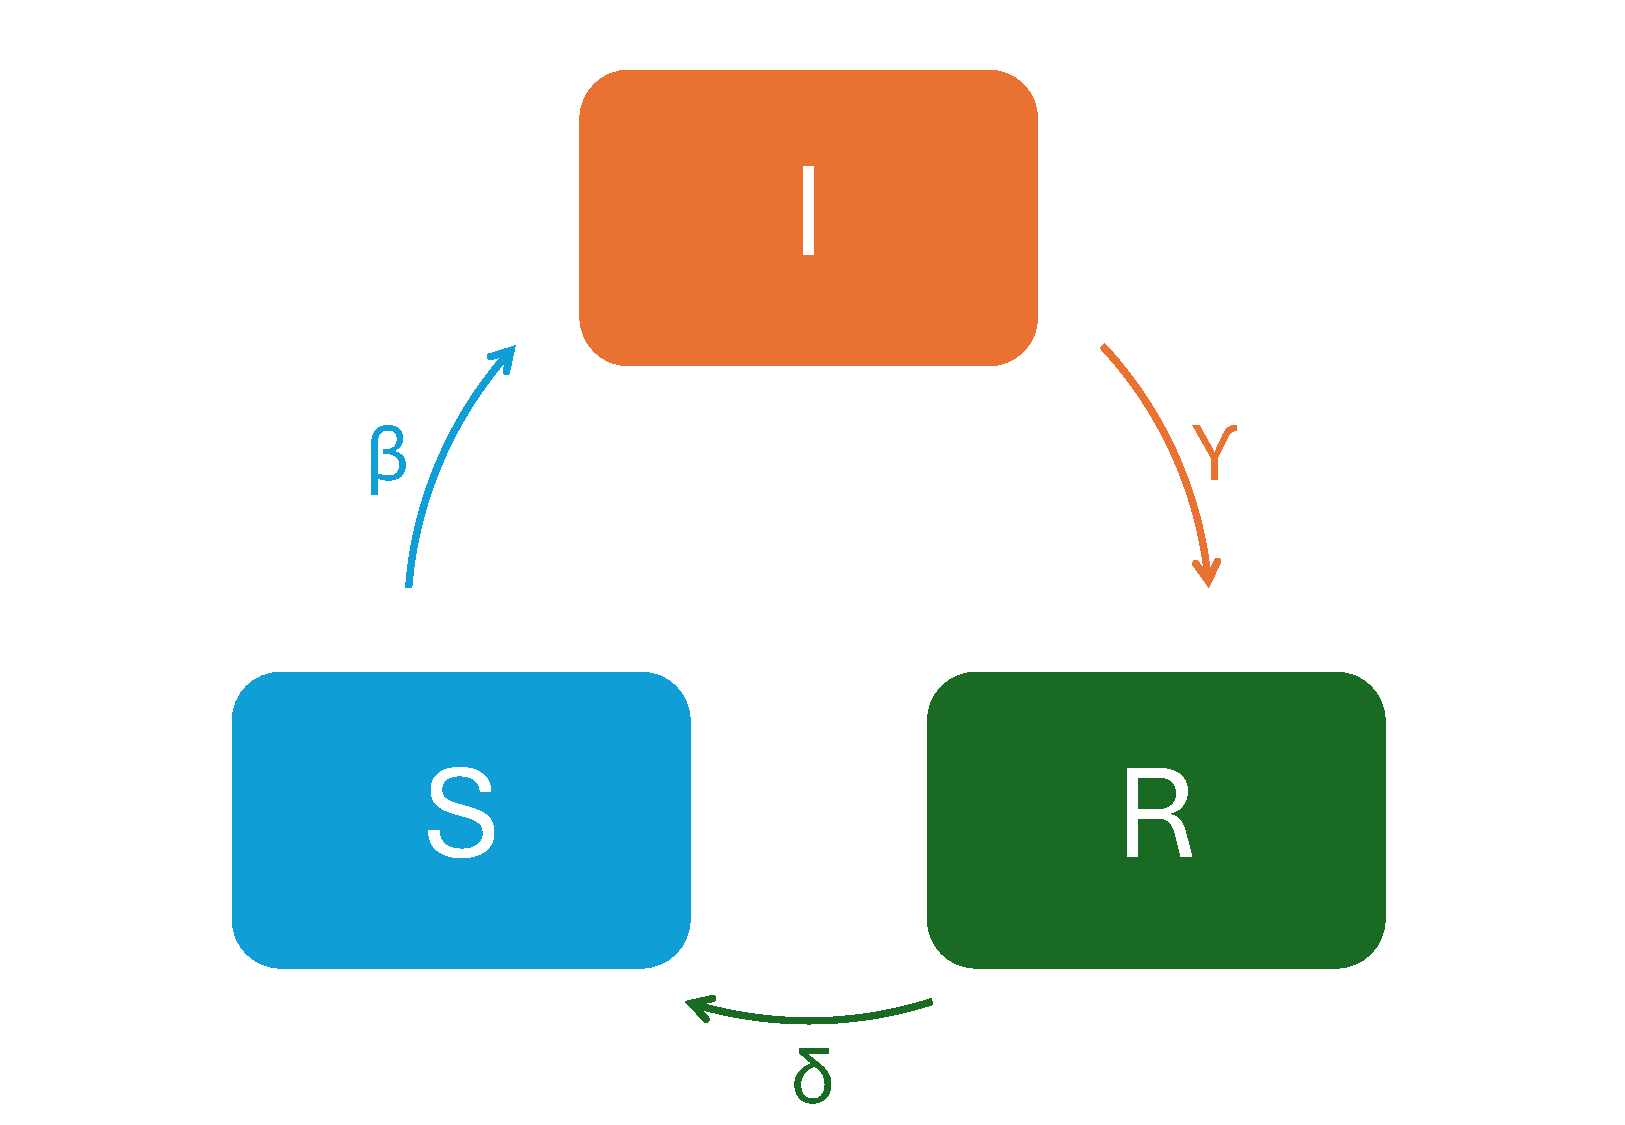
\includegraphics[width=0.65\linewidth]{0_introduction/images_introduction/SIRS_figure_compartmental}
	\caption[SIRS example]{An example of the graph structure of a mean field SIRS model. There are three compartments and the flow rate between them is ruled by the coefficients $\beta$, $\gamma$ and $\delta$.}
	\label{fig:sirsfigurecompartmental}
\end{figure}


\subsubsection{SIR model}
\label{subsec:SIR}
The foundational model for studying epidemics mathematically is the SI model. In this model, the population is divided into two compartments: Susceptible $(S)$ and Infected $(I)$. Individuals transition from being susceptible to infected, but there is no recovery, meaning once infected, individuals remain infectious indefinitely.

An extension of this is the SIR model, which adds a third compartment, Recovered $(R)$. This additional compartment represents individuals who have either gained immunity or have died, removing them from the cycle of infection. After spending a certain period in the infected state, individuals transition to the recovered state, making them no longer susceptible to the disease.
Now to begin introduce the SIR model structure, first its compartments subdivision is pressented. The population or density of individuals is sub-divided into three groups: Susceptible, Infectious, and Recovered. At time $t$ the three groups are identified with the symbols: $S(t)$, $I(t)$, and $R(t)$. 
The symbols used to indicate the density of each group are instead $s$, $i$, and $r$, while the capital letters are used to specify both the name of the groups or the absolute number of participants in each one. 

The SIR model, which will be described in the following sections, is built upon several assumptions that shape the mathematical framework. These guiding principles are introduced in the following paragraphs. Furthermore, the main properties of the model will also be introduced. 

\subsubsection{Mean-field approximation}
The approximation that gives the name to this model class is based on a method that permits the analytical analysis of complex systems. With mean-field, individual-level interactions are averaged, focusing not on individual behavior but on the collective behavior of the population. Using this method, equations can be derived that describe disease evolution in terms of average rates rather than tracking individual agents.
\subsubsection{Homogeneus mixing} 
It is the assumption that all individuals in the population mix homogeneously, meaning that the probability of interacting with any individual is the same. It is a strong assumption because it implies ignoring any spatial or social structure.
\subsection{Average rates of changes}
\label{sec:sir_presentation}
In the model, differential equations are used to represent the transition of individuals between different compartments. These transitions can depend on the state of the system but, in the simplest form, are based on average rates. The three rates used in the SIRS mean-field model are:
\begin{itemize}
	\item $\beta$: transmission rate;
	\item $\gamma$: recovery rate;
	\item $\delta$: waning immunity rate.
\end{itemize}
The flow of individuals in the system is shown in Figure \ref{fig:sirsfigurecompartmental}.

\subsubsection{Population being constant}
The total population size, represented by the letter $N$, is the sum of individuals in the three compartments (e.g., Susceptible, Infected, and Recovered). It is often assumed to remain constant during the course of an epidemic. This assumption is based on the idea that epidemics typically last much shorter than the average human lifespan, making the effects of births and deaths negligible.
In more complex models, where demographic effects are considered, such as in models of longer-lasting epidemics, the population size can still be assumed constant by balancing the number of births (modeled as an influx into the Susceptible compartment) with the number of deaths (modeled as an outflux). This approach assumes that births and deaths occur at approximately the same rate, keeping the total population size stable over time. The result of this assumption implies that:
\begin{itemize}
	\item Population density compartments sum up to one.
\end{itemize}
\[s(t) + i(t) + r(t)= 1 \]
\begin{itemize}
	\item The sum of the derived functions w.r.t. time is equal to zero.
\end{itemize}
 \[\dot{s}(t)+ \dot{i}(t) + \dot{r}(t)= 0\]

\subsubsection{Recover transition} 
The first fundamental dynamic process of the model assumes that the infected compartment decreases in size, with a rate of decrease proportional solely to the current number of infected individuals. This gives the following relation:
\[\frac{d i}{dt} = - \gamma i, \qquad i(0) = i_0, \]
which models a continuous process. Specifically, it assumes that individuals transition from the infectious state to the recovered state at a constant rate, denoted by $\gamma$. The physiological meaning of this parameter is that it represents the inverse of the infection's duration, meaning that the average infection lasts $1/\gamma$ days. Thus, $\gamma$ is the recovery rate, reflecting the speed at which the population recovers from the disease.
 
%In this model the disease reproduces through horizontal incidence, and so the contagion is modeled as due to random contact that happens in a homogeneosuly mixed population.
\subsubsection{Person-to-person disease transmission}
\label{subsubsec:p2p_transmission}
To model this quantity fractional terms are used, assuming a population composed of susceptible and infected individuals. Each infectious individual encounters a fraction $c$ of the population per day. If all encounters are equally likely, a fraction $s$ of these encounters will be with susceptibles. Therefore, each infectious individual has $c\cdot s$ encounters with susceptibles. The probability that an encounter leads to transmission is $p$, meaning the average number of transmissions per day is $p \cdot c \cdot s$. Considering the fraction of infected individuals $i$, and combining $p$ and $c$ into a single parameter $\beta$, the transmission rate becomes:
\[\text{transmission rate} = \beta s i.\]
Here, $\beta$ represents the transmission coefficient.


\subsubsection{Immunity}
In SIR model, once individuals recover from the disease, there are no further transitions. Two possible model scenarios can cause this:
\begin{itemize}
	\item Lifelong immunity acquired after recovery, ini this case the meaning of the compartments is $R =$ recovered.
	\item Death of infected individuals, here the compartments can be intended as $R =$ removed.
\end{itemize}
Both cases assume that, once the illness period ends, the disease can no longer be transmitted.
If immunity acquired from an infection wanes after a certain period, individuals can become susceptible again, leading to an SIRS model. The $\delta$ rate is used to express the outflow from the Recovered compartment, and it corresponds to the inverse of the average duration of immunity.

\subsubsection{Threshold value}
\label{subsub:threshold}
Although the SIR model is simple, it plays a fundamental role in predicting a key aspect of epidemics: the threshold value, a concept first introduced by Kermack and McKendrick in their pioneering work \cite{kermack1927}. They showed that, in a fully susceptible population, an epidemic will only start if the basic reproduction number $\mathcal{R}_0$ is greater than $1$, marking the birth of the term "threshold value" in epidemiology.
In the SIR model the reproduction number value is equal to the ratio between the transmission and recovery rate:
\begin{equation}
	\mathcal{R}_0 = \frac{\beta}{\gamma}. 
	\label{eq_basic_reproduction_number}
\end{equation}

Over the years, the dynamics of this system have been extensively studied and analyzed \cite{Breda_2012, akinboro2014numerical, Jard_n_Kojakhmetov_2021, Ledder_2023, Okabe_2020, Prodanov_2022, Xu_2014, Turkyilmazoglu_2021}. The threshold effect highlights two distinct scenarios:
\begin{itemize}
	\item \textbf{Free Disease Equilibrium $(\mathcal{R}_0 < 1)$:} When $\mathcal{R}_0$ is less than one, the disease does not spread within the population. Although infected individuals make contact with susceptibles, the rate of disease transmission is slower than the recovery rate. Mathematically, this means $\beta / \gamma < 1$, or $\beta < \gamma$, where $\beta$ represents the transmission rate and $\gamma$ the recovery rate. Consequently, the healing process is faster than the spread of infection, and the number of infected individuals quickly drops to zero. The majority of the population remains susceptible, and this state is globally asymptotically stable, as demonstrated by \cite{Hernandez_Vargas_2022}.
	\item \textbf{Epidemic spread $(\mathcal{R}_0 > 1)$:}     When the threshold is greater than one, the number of infected individuals grows until it reaches a peak and then declines toward zero. The peak number of infected people, as well as the final number of susceptibles, can be calculated using the system's initial conditions and the values of $\beta$ and $\gamma$, as described by \cite{Hethcote_2000}. 
	As reported in this work:
	\begin{quotation}\small
	Let $s_s(t),i_s(t)$ be a solution of the system 
	\begin{equation}
		\begin{split} 
			ds/dt &= -\beta i s\\
			di/dt &= \beta i s - \gamma i	
		\end{split}
	\end{equation}

	with $s(0) = s_0 \ge 0$, and $i(0) \ge 0$. The mass conservation assumption holds so $r(t) = 1-s(t)-i(t)$. The triangle in the $si$ phase plane given by 
	\[T ) {(s,i)|s \ge 0, i\ge 0, s+i \le 1 }\]
	is positively invariant and unique solutions exist in $T$ for all positive time, so that the
	model is mathematically and epidemiologically well posed.
	If parameter $\sigma$ is defined as $\sigma=\beta/\gamma$ it holds that if $\sigma s_0 >1$, the $i(t)$ first increase up to a maximum value $i_{max} = i_0 + s_0 - 1/\sigma - [\log(s_\infty/s_0)]/\sigma $ and then decrease to zero as $t \rightarrow \infty$. The susceptible fraction $s(t)$ is a decreasing function and the limiting value $s_\infty$ is the
	unique root in $(0, 1/\sigma)$ of the equation
	\[
	i_0 + s_0 -s_\infty - \log(s_\infty/s_0)/\sigma = 0. 
	\]		
	\end{quotation}
	
	This scenario illustrates how a highly aggressive infection can spread widely within a population. If no countermeasures are taken, it can lead to significant social and economic consequences. A typical epidemic outbreak has an infective curve that first increases from an initial Io near zero, reaches a peak, and then
	decreases toward zero as a function of time. The susceptible fraction $s(t)$ instead always
	decreases, but the final susceptible fraction $s_\infty$ is positive. The epidemic dies out because, when the susceptible fraction $s(t)$ goes below $1/\sigma$, the replacement number $\sigma s(t)$ goes below 1.
		
\end{itemize}
	Thus, even with its simplicity, the SIR model provides critical insights into the potential severity of an epidemic and highlights the importance of timely interventions to prevent widespread harm.
	

\subsubsection{The SIR mean-field model equations}
After introducing the basic framework of the model, the set of differential equations that describe the rates of change in the system's state is presented. The equations, along with initial conditions, are necessary to fully define the model. The class sizes are expressed as fractions of the total, constant population.

The model is then
\begin{equation}
	\begin{cases}
		ds(t) / dt = -\beta s(t) i(t), \;\qquad \qquad s(0) = s_0 \gg 0;\\
		di(t) / dt =  \beta s(t) i(t) - \gamma i(t), \qquad i(0) = i_0 > 0;\\
		dr(t) / dt =  \gamma i(t), \qquad \; \, \;\quad \quad \qquad r(0) = r_0 = 0;
	\end{cases}
\end{equation}
where
\begin{equation}
s_0 + i_0 + r_0 = 1.
\end{equation}

Several works analyze this model and provide a detailed mathematical derivation of its solution \cite{diekmann2000mathematical,akinboro2014numerical,Turkyilmazoglu_2021}. However, this is not the focus of the present work. Instead, we provide an overview of the main results and a summary of the dynamics that emerge from the model.

\subsubsection{Model behavior}

To present the evolution of the model, a simple numerical simulation is carried out. The removal rate is set to $\gamma = 0.1$, meaning the infection lasts, on average, 10 days. The transmission rate is $\beta = 0,5$. At the start of the simulation, the majority of the population is in the susceptible class, with only a small portion of individuals already infected.

The initial reproduction number is  $\mathcal{R}_0 = 5$, which is greater than 1. As discussed in Section \ref{subsub:threshold}, this indicates that the disease will evolve into an epidemic.

The key features that emerge from the model simulation are:

\begin{itemize}
	\item \textbf{Slow initial phase:} The early stages of the epidemic are marked by a slow start, as seen in the first part of the curves in Figure \ref{fig:sir_example0}a. The curves remain nearly flat because only a few individuals are initially infected, and it takes time for the infection to spread and reach a larger portion of the population.
	\item \textbf{Exponential growth:} In the second stage, the number of infections increases exponentially.
	\item \textbf{Peak infection:} Eventually, the number of infections reaches a peak.
	\item \textbf{Residual susceptible population:} By the end of the epidemic, a portion of the population remains susceptible, though this amount depends on the model's parameters.
\end{itemize}

An additional detail emerging from the model, as analyzed in \cite{Okabe_2020} and visible in Figure \ref{fig:sir_example0}, is the evolution of the reproductive ratio over time. The reproductive ratio is given by the formula $\mathcal{R}(t) = \frac{\beta}{\gamma} \cdot s(t)$. Initially, assuming $s(0)\approx 1$, we can simplify this to obtain the value of $\mathcal{R}_0$. However, as the susceptible fraction decreases exponentially alongside the growth in infections, the reproductive ratio also decreases, and the infection peak occurs when $\mathcal{R}(t)=1$.


\begin{figure}[ht]
	\centering
	\subfloat[][\emph{}]
	{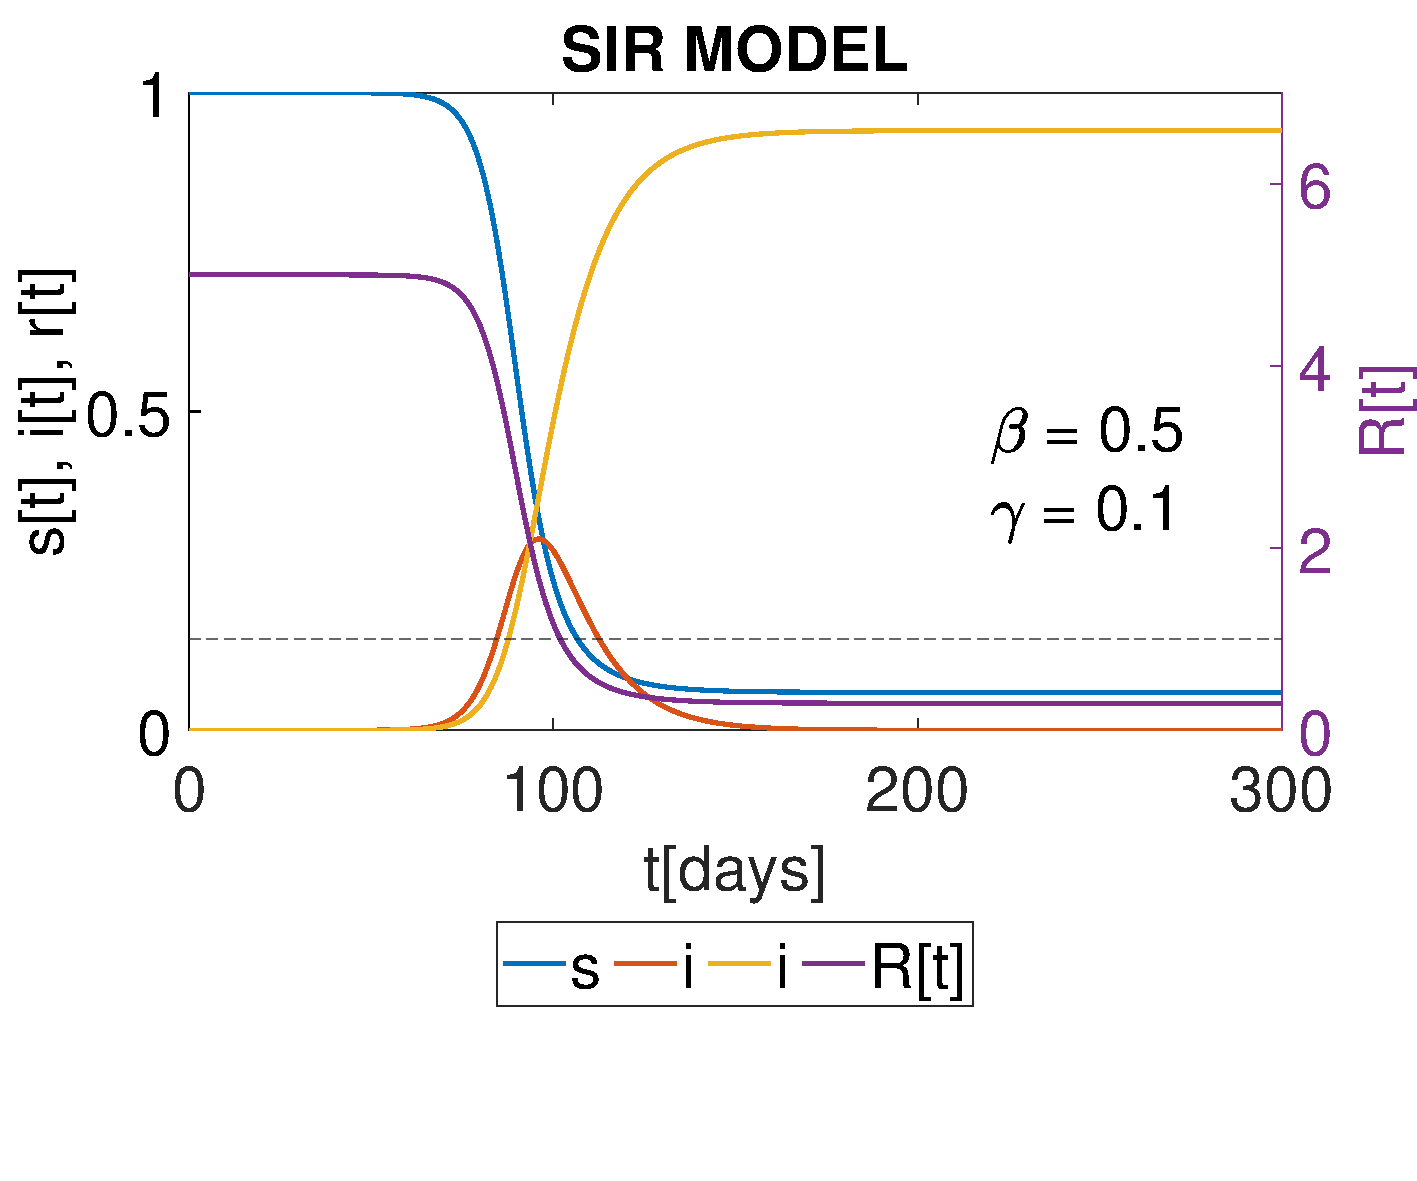
\includegraphics[width=0.48\linewidth]{0_introduction/images_introduction/sir_con_rt}} \quad
	\subfloat[][\emph{}]
	{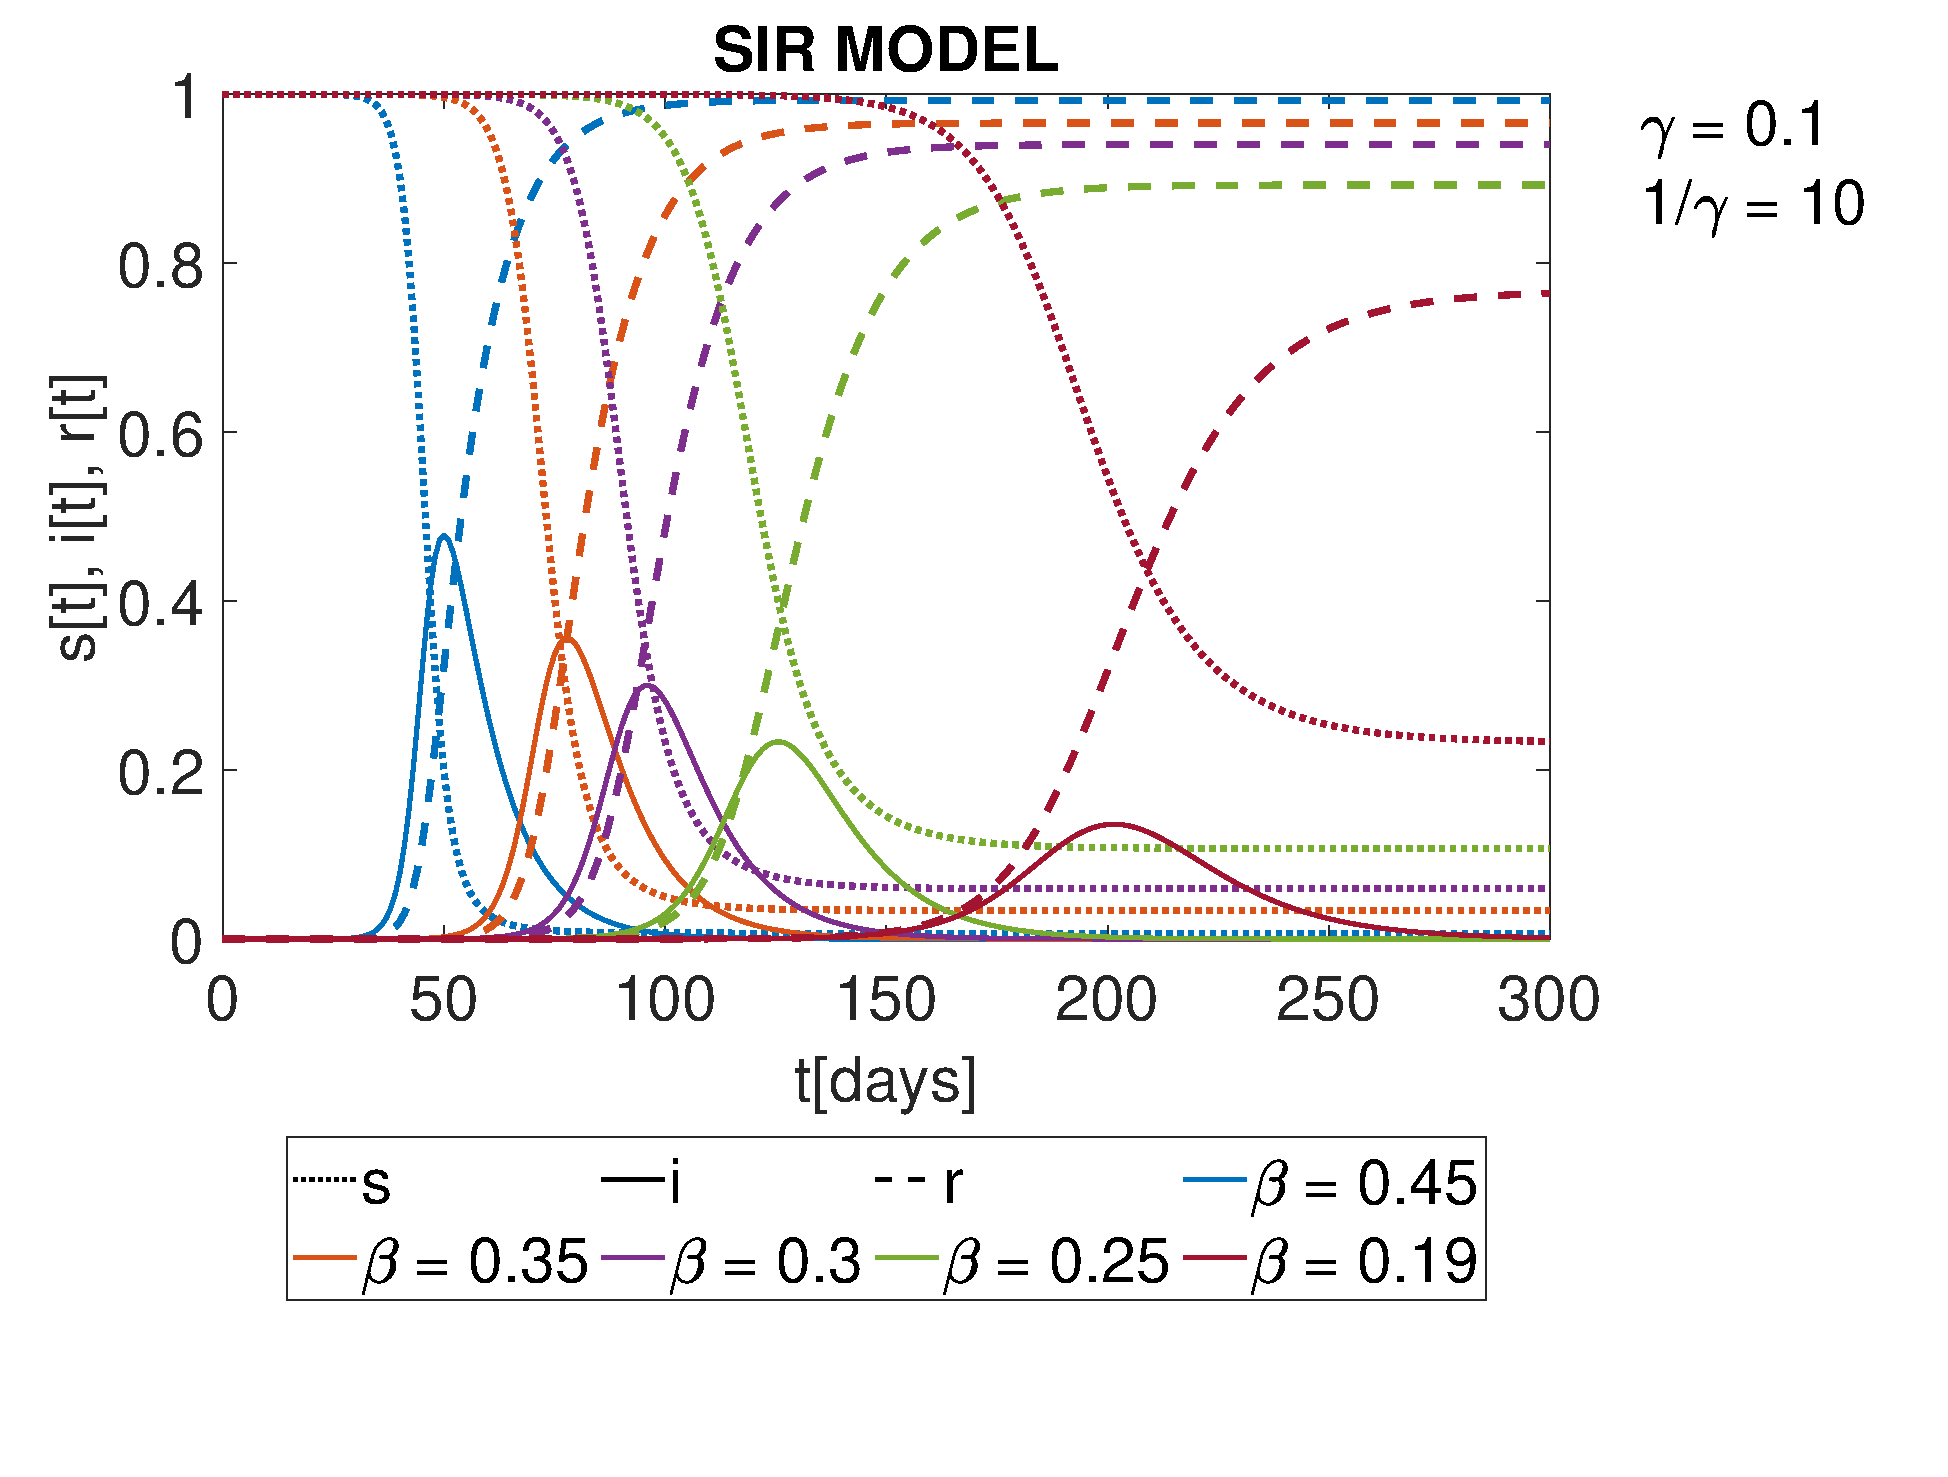
\includegraphics[width=0.48\linewidth]{0_introduction/images_introduction/sir_multipli_beta}} \\
	\caption[SIR dynamic example]{SIR system numerical solutions. Figure a) shows the evolution of compartments in the case of an epidemic. The violet dotted line represents the time-dependent $\mathcal{R}_0(t)$. It can be seen that when this parameter is equal to $1$, the number of infected reaches its maximum value. In b) are presented different evolutions of the disease varying only the $\beta$ coefficient. The smaller its value the flattened and the more delayed the infectious curve is.}
	\label{fig:sir_example0}
\end{figure}
Two key metrics to consider during the emergence of a new disease are the rate of increase of infections and the final size of the remaining susceptible population by the end of the epidemic. The course an epidemic takes can vary dramatically depending on whether it spreads rapidly, overwhelming healthcare systems, or whether interventions succeed in "flattening the curve."
The rate of infection growth depends on how quickly the disease spreads through the population. If an epidemic grows rapidly, a large number of people fall ill in a short period, potentially overwhelming healthcare resources.
On the other hand, the final size of the susceptible population indicates how many individuals remain uninfected once the epidemic has run its course. This is influenced by factors such as herd immunity or interventions like vaccination.
"Flattening the curve" refers to strategies aimed at slowing the spread of the disease, thereby reducing the peak number of infections and spreading cases over a longer period. This reduces the strain on healthcare systems without necessarily reducing the total number of infections.

Some strategies for flattening the curve include:
\begin{itemize}
	\item Social distancing and quarantine to reduce contact between susceptible individuals and the infected. This decreases the transmission rate $\beta$.
	\item Vaccination, which immediately reduces the number of susceptible individuals, thus preventing the disease from spreading widely.
\end{itemize}
While flattening the curve may not lower the total number of infections (i.e., the cumulative number may remain the same), it reduces the peak number of active cases at any given time, which is crucial for ensuring that healthcare systems are not overwhelmed.


\subsection{Other modeling techniques}
There are several ways to model an epidemic, and the main categories of these models are now introduced. Many of the articles that will be reviewed in the next chapter \ref{ch:literature_review} make use of one or more of these model types.
\subsubsection{Stochastic models} 	
This group of models, which originate from the mean-field approach, utilizes a different mathematical framework. In these models, the transition between states is governed by stochastic functions. Conceptually, they share the same foundation as ordinary differential equation (ODE) models but differ in application. These stochastic models are particularly useful when studying diseases with a lower number of infected individuals or when the epidemic's outcome is influenced by changes in individual dynamics, a phenomenon known as demographic variability. Demographic variability includes changes in transmission rates, birth rates, recovery rates, or mortality within the population.
One approach to model such variability is through stochastic models paired with Monte Carlo simulations \cite{Allen2017}.

\subsubsection{Networked models}
In this class of models, disease dynamics are considered over complex and realistic networks, with a focus on understanding how the network structure impacts the epidemic's spread by analyzing parameters like the rate of infection. The model represents individuals as nodes in a graph, with edges illustrating interactions between them. Nodes can also represent subgroups, and the relationships between individuals or groups can be weighted, representing varying strengths of interactions \cite{Newman2002,VanMieghem2009}. The larger the number of nodes and the more accurately the connections reflect real-world interactions, the better the model is at reliably simulating the spread of the disease.


\subsubsection{Agent-based models}
Agent-based models (ABMs) simulate the progression of a disease by focusing on the behavior and interaction of autonomous agents, which could be individuals or collective entities like organizations. This modeling approach is built on observing spontaneous interactions between individuals \cite{Tizzoni2014}, creating a dynamic system where each person acts according to certain rules. The goal is to understand how these individual behaviors influence the overall evolution of the system.

One key advantage of ABMs is that they provide an intuitive way to interpret epidemic modeling by focusing on individual perspectives, making the model's results easier to understand. Additionally, because agents embed individual behavior, ABMs can deliver highly detailed simulations and offer insights into specific countermeasures that might help mitigate the spread of a disease.

However, ABMs require a large amount of detailed, reliable data to be effective, as their accuracy depends on the precision of the information integrated into the model. Collecting and incorporating this data can be a challenging task, which is a potential limitation of this modeling approach \cite{Hernandez_Vargas_2022}.
\begin{figure}
	\centering
	
\includegraphics[width=0.5\linewidth]{0_introduction/images_introduction/agent_based}
	\caption[Agent based network representation]{Agent based network representation}
	\label{fig:agentbased}
\end{figure}

\subsubsection{Multilayer systems and networks} 
The complex dynamic of interactions existing in the real world, develops in multiple patterns, with complicated relationships. These interactions can change over time, and using the theory of multilayer systems can improve the comprehension of such complexity. Additional information can be added to the model, for example, different types of interactions, like physical contact or information sharing, time dependency coefficients, or reliance between different parameters in nature, creating cause-effect relationships.
\begin{figure}[ht]
	\centering
	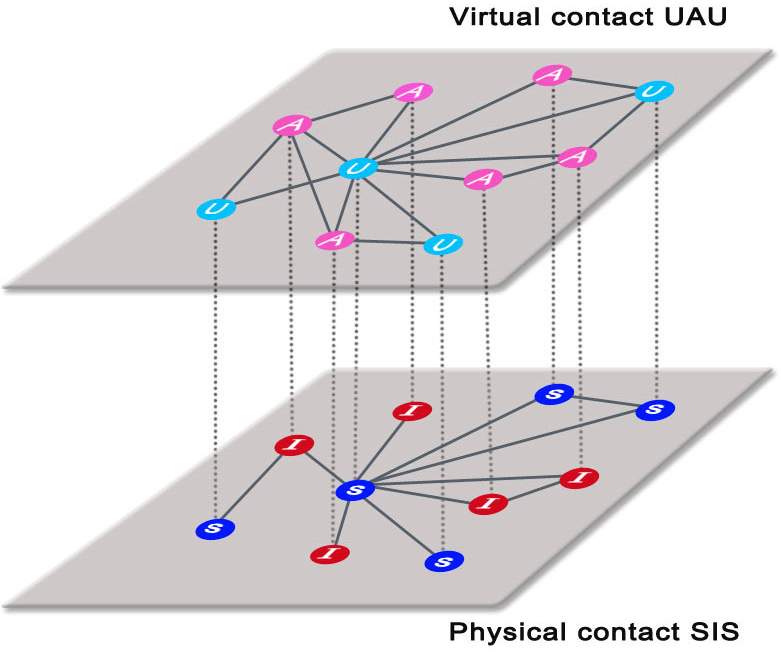
\includegraphics[width=0.5\linewidth]{0_introduction/images_introduction/multi_layer}
	\caption[Multi-layer network]{Representation of a multiplex structure. The figure is taken from the work of \cite{Granell2013} and shows the network implemented in their model. There are two layers coupled together: one representing awareness and the other the epidemic state. In this case, nodes connected by interlayer connections represent the same individual. Thus, the model describes people with two attributes: awareness of a disease and health state. The mechanisms of infection and becoming aware are distinct, but both attributes influence how an agent's state evolves. For example, if an agent is aware of the disease, they may act more cautiously, thereby reducing their probability of becoming infected.}
	\label{fig:multilayer}
\end{figure} 
In a more recent development of the research, the traditional network theory was revisited, to create a framework that can include multiple networks, that evolve and influence each other \cite{DeDomenico2016, Krickel_2023} and can be helpful to describe complex systems like human relationships. An interesting result obtained is the possibility that the onset of one disease can depend on the onset of the other one. There can be regimes in which the criticality of the two dynamics is interdependent and others in which the critical effect is only one-directional \cite{DeDomenico2016}. 
One possible way to develop models with this structure is to imagine that each layer represents a different type of interaction. An epidemiological example is a model that considers, for each agent, both its physical contacts with others, where the disease can be transmitted, and its network of relations, representing the social dynamics in which everyone is involved. An example of this network is shown in Figure \ref{fig:multilayer}. This instrument provides a natural representation of coupled structure and dynamical processes. It has been presented in multiple works in the past years, for example in \cite{Wang_2019}. 
Multiple systems can have either a single or coupled dynamic. In the case of a single dynamic, there is a top layer whose evolution occurs independently on top of a multilayer network. In contrast, a coupled structure describes phenomena in each layer evolving under the mutual influence of what is happening in the other layers.


%%%%%%%%%%%%%%%%%%%%%%%%%%%%%%%%%%%%%%%%%%%%%%%%%%%%%%%%%%%%%%%%%%%%
